\documentclass[11pt,a4paper]{article}
\usepackage[margin=22mm]{geometry}
\usepackage{fontspec}
\usepackage{amsmath,amssymb,booktabs,graphicx,float,array,enumitem,xcolor,hyperref}
\hypersetup{colorlinks=true,linkcolor=blue!50!black,urlcolor=blue!50!black,
  pdftitle={Q1: Three bosons on a 2D lattice}}
\setlist{itemsep=2pt,topsep=3pt,leftmargin=1.8em}
\setlength{\parskip}{4pt}
\setlength{\parindent}{0pt}
\linespread{1.1}
\newenvironment{keybox}[1]
  {\par\noindent\setlength{\fboxsep}{8pt}\setlength{\fboxrule}{0.6pt}%
   \begin{lrbox}{0}\begin{minipage}{\dimexpr\linewidth-2\fboxsep-2\fboxrule\relax}%
   {\bfseries\color{blue!45!black}#1}\par\smallskip}
  {\end{minipage}\end{lrbox}\fcolorbox{blue!45!black}{blue!3}{\usebox{0}}\par}
\newcommand{\Etwo}{-0.820776322}
\newcommand{\Eground}{-4.771434366}
\newcommand{\Eexcited}{-1.108993749}
\newcommand{\Erel}{-0.288217427}
\newcommand{\Binding}{3.950658045}
\newcommand{\CstarMax}{4.2910935}
\newcommand{\Lmax}{40}
\newcommand{\LastRootChange}{0.000982}
\newcommand{\RmsGround}{0.673}
\newcommand{\RmsExcited}{2.144}
\newcommand{\MaxResidual}{7.31\times10^{-11}}
\newcommand{\MaxSymmetry}{1.13\times10^{-10}}
\newcommand{\MaxOrtho}{1.49\times10^{-14}}
\newcommand{\Nsolves}{152}

\newcommand{\rr}{\mathbf r}
\newcommand{\dd}{\boldsymbol\delta}
\newcommand{\Ethr}{E_{\mathrm{thr}}}

\begin{document}

\begin{center}
{\LARGE\bfseries Q1: From $^8$Be to a Toy Carbon Nucleus}\\[6pt]
{\large Derivation, solution and verification of a three-boson lattice model}\\[4pt]
{\small TIF345/FYM345 \quad Project: \textit{Fine-tuned for life?}}
\end{center}

\begin{keybox}{The question (Q1, verbatim)}
\textit{Compute the threshold and the $0^+_1$ and $0^+_2$ states (a sparse eigensolver in the full space suffices),
and verify their symmetry. How do they and the threshold depend on $c\in[3.5,7]$ and $L$, and at which $c^\star$
does the Hoyle-like state cross the threshold? How do you know that your results are right?}

\medskip
\textbf{Answer at a glance.}
(1) At $c=5,L=20$: $\Ethr=-0.821$, $E_{3,1}=-4.771$, $E_{3,2}=-1.109$, reproducing the benchmark.
(2) All levels decrease monotonically with $c$; the Hoyle-like state falls faster than the threshold and therefore crosses it from above.
(3) The crossing depends on the box size and converges to $c^\star\approx4.29$ in large boxes.
(4) Analytic limits, symmetry, derivative and convergence checks together establish correctness.
\end{keybox}

%====================================================================
\section{Theory}

\subsection{Model}
Three identical bosons of mass $m$ live on a periodic $L\times L$ lattice with spacing $a$:
\begin{equation}
H=-\frac{\hbar^2}{2m}\sum_{i=1}^{3}\nabla_i^2+\sum_{i<j}V_c(|\mathbf x_i-\mathbf x_j|),\qquad
V_c(r)=-c\,\underbrace{e^{-r^2}}_{f(r)}+\underbrace{\frac{0.3}{\sqrt{r^2+1}}}_{g(r)}.
\end{equation}
$f$ is a short-range attraction of strength $c$ (the ``strong force''), $g$ a weak long-range repulsion (``Coulomb'').
We write $t=\hbar^2/(2ma^2)$ and set $a=t=1$ numerically.
Distances use the minimum image, $d_L(\rr)=\min_{\mathbf n\in\mathbb Z^2}|\rr+La\,\mathbf n|$.

\subsection{Step 1: kinetic energy on the lattice}
Adding the Taylor expansions of $\phi(x\pm a)$ cancels the odd orders:
\begin{equation}
-\frac{\hbar^2}{2m}\phi''(x)=t\,[2\phi(x)-\phi(x+a)-\phi(x-a)]+O(a^2).
\end{equation}
With the periodic shift $(S\phi)_n=\phi_{(n+1)\bmod L}$ the 1D kinetic matrix is $t(2I-S-S^T)$; in 2D, with $S_x=S\otimes I$, $S_y=I\otimes S$,
\begin{equation}
(T_1\phi)(\mathbf x)=4t\,\phi(\mathbf x)-t\sum_{\dd}\phi(\mathbf x+\dd),\qquad \dd\in\{\pm\hat x,\pm\hat y\}.
\end{equation}
\textbf{Rule of thumb:} each particle contributes $4t$ on the diagonal and $-t$ for each nearest-neighbour hop; the potential is diagonal in the position basis.

\subsection{Step 2: translation invariance $\Rightarrow$ relative coordinates}
A global shift $\mathbf x_i\mapsto\mathbf x_i+\mathbf b$ preserves both hops and pair distances, so it commutes with $H$ and the total momentum $\mathbf K$ is conserved.
We need only the centre-of-mass-at-rest block $\mathbf K=0$, where the wave function depends on relative coordinates alone.
This reduces the dimension from $L^{2n}$ to $L^{2(n-1)}$.

\paragraph{Two bodies.} Let $\rr=\mathbf x_1-\mathbf x_2$ and $\Psi(\mathbf x_1,\mathbf x_2)=\phi(\rr)$.
A hop $\dd$ of particle 1 gives $\phi(\rr+\dd)$, a hop of particle 2 gives $\phi(\rr-\dd)$; since $\{\dd\}$ is symmetric, the two sums coincide:
\begin{equation}
\boxed{(H_2\phi)(\rr)=8t\,\phi(\rr)-2t\sum_{\dd}\phi(\rr+\dd)+V_c\big(d_L(\rr)\big)\,\phi(\rr)}
\label{eq:h2}
\end{equation}
The hopping amplitude $2t$ reflects the reduced mass $\mu=m/2$. The matrix has dimension $L^2$.

\paragraph{Threshold.} ``Two-body bound state plus a particle at rest'' costs the two-body ground-state energy plus zero:
\begin{equation}
\Ethr=E_2=\min\operatorname{spec}(H_2),\qquad
E_R=E_{3,2}-\Ethr,\qquad B=\Ethr-E_{3,1},\qquad E_R(c^\star)=0.
\end{equation}

\paragraph{Three bodies.} Let $\rr_1=\mathbf x_1-\mathbf x_3$, $\rr_2=\mathbf x_2-\mathbf x_3$. One hop of each particle does:
\begin{center}
\begin{tabular}{lll}
\toprule
Particle hop & $(\rr_1,\rr_2)$ becomes & \\
\midrule
$\mathbf x_1\to\mathbf x_1+\dd$ & $(\rr_1+\dd,\ \rr_2)$ & moves $\rr_1$ only \\
$\mathbf x_2\to\mathbf x_2+\dd$ & $(\rr_1,\ \rr_2+\dd)$ & moves $\rr_2$ only \\
$\mathbf x_3\to\mathbf x_3+\dd$ & $(\rr_1-\dd,\ \rr_2-\dd)$ & \textbf{moves both} \\
\bottomrule
\end{tabular}
\end{center}
The diagonal kinetic term is $3\times4t=12t$, and there are $3\times4=12$ hops:
\begin{equation}
\boxed{\begin{aligned}
(H_3\psi)(\rr_1,\rr_2)={}&12t\,\psi-t\sum_{\dd}\Big[\psi(\rr_1{+}\dd,\rr_2)+\psi(\rr_1,\rr_2{+}\dd)+\psi(\rr_1{-}\dd,\rr_2{-}\dd)\Big]\\
&+\Big[V_c\big(d_L(\rr_1)\big)+V_c\big(d_L(\rr_2)\big)+V_c\big(d_L(\rr_1-\rr_2)\big)\Big]\psi
\end{aligned}}
\label{eq:h3}
\end{equation}
The diagonal hop comes from particle 3; it is the lattice counterpart of the cross term in the continuum kinetic energy
$-\tfrac{\hbar^2}{m}(\nabla_1^2+\nabla_2^2+\nabla_1\!\cdot\!\nabla_2)$.

\begin{figure}[H]
\centering
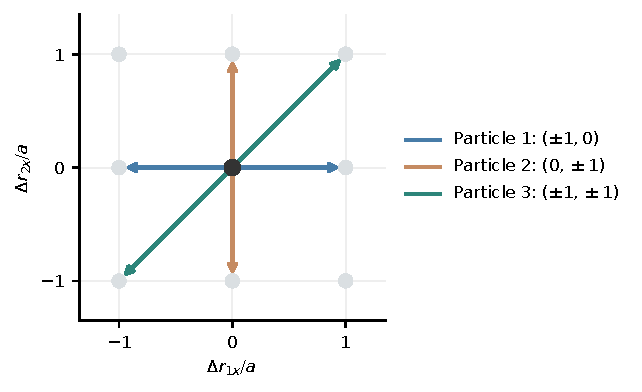
\includegraphics[width=.62\textwidth]{../figures/relative_hops.pdf}
\caption{Hop directions in relative coordinates ($x$ components; $y$ is analogous). The green diagonal hops come from particle 3.}
\end{figure}

\paragraph{Matrix form.} The whole problem reads
\begin{equation}
H(c)=T+G-c\,F,
\end{equation}
with sparse kinetic $T$ and diagonal potentials $F,G$ (summed over pairs). $H$ is \textbf{real symmetric};
the three-body matrix has dimension $L^4$ but only 13 non-zeros per row. $T,F,G$ do not depend on $c$, so changing $c$ only changes the diagonal.

\subsection{Step 3: symmetry and the meaning of $0^+$}
$H$ has two kinds of symmetry, both permutations of configurations:
\begin{itemize}
\item \textbf{Boson exchange $S_3$}, generated by $P_{12}:(\rr_1,\rr_2)\mapsto(\rr_2,\rr_1)$ and
      $P_{13}:(\rr_1,\rr_2)\mapsto(-\rr_1,\ \rr_2-\rr_1)$ (substitute $\mathbf x_1\leftrightarrow\mathbf x_3$).
\item \textbf{Lattice point group $D_4$}, generated by $R_{90}:(x,y)\mapsto(-y,x)$ and $M_x:(x,y)\mapsto(x,-y)$, acting on $\rr_1,\rr_2$ simultaneously.
\end{itemize}
They map hops to hops and pairs to pairs and preserve $d_L$, hence $[H,\mathcal S]=0$.
A square lattice has no continuous rotations; the lattice analogue of $0^+$ is a state that is fully symmetric under $S_3$ and in the trivial irrep $A_1$ of $D_4$.
Invariance under the generators implies invariance under the whole group:
\begin{equation}
\psi\in0^+\iff \mathcal S\psi=\psi,\qquad \mathcal S\in\{P_{12},P_{13},R_{90},M_x\}.
\end{equation}
For a normalised real eigenvector in another one-dimensional irrep some $\|\mathcal S\psi-\psi\|=2$; two-dimensional irreps also give $O(1)$.
Symmetric and non-symmetric states are therefore separated by orders of magnitude.

\subsection{Step 4: how levels depend on $c$}
For a non-degenerate normalised eigenstate the Hellmann--Feynman theorem gives
\begin{equation}
\frac{\partial E_n}{\partial c}=\Big\langle\frac{\partial H}{\partial c}\Big\rangle_n=-\langle F\rangle_n\le0 .
\end{equation}
Since $F\ge0$, \textbf{stronger attraction lowers every level}. However,
$\dfrac{dE_R}{dc}=-\langle F_3\rangle_{0^+_2}+\langle F_2\rangle_{2}$ has a sign set by which expectation value is larger; it must be computed---this is the essence of the crossing question.
$H(c)$ is linear in $c$, so non-degenerate eigenvalues are smooth; if $E_R$ changes sign on an interval, the intermediate value theorem guarantees a root $c^\star$ inside.

\subsection{Step 5: two analytic handles}\label{sec:analytic}
\paragraph{Free spectrum.} Set $V=0$ and insert the plane wave $\psi=e^{i(\mathbf k\cdot\rr_1+\mathbf q\cdot\rr_2)}$ into \eqref{eq:h3}:
\begin{equation}
T_3\psi=\big[\epsilon(\mathbf k)+\epsilon(\mathbf q)+\epsilon(\mathbf k+\mathbf q)\big]\psi,\qquad
\epsilon(\mathbf k)=2t\sum_{\mu}[1-\cos(k_\mu a)],
\end{equation}
exactly the free energy of three particles with momenta $\mathbf k,\mathbf q,-(\mathbf k+\mathbf q)$; for two bodies one gets $2\epsilon(\mathbf k)$.
Dropping the diagonal hop, or using $t$ instead of $2t$ for two bodies, breaks this identity, so it tests the derivation directly.

\paragraph{Finite volume.} A bound state decays as $\psi\sim e^{-\kappa r}$ with $\kappa\propto\sqrt{|E_{\rm bind}|}$.
The periodic box makes it overlap with its images, giving corrections $\Delta E(L)\sim e^{-\kappa La}$: \textbf{the looser the state, the slower the convergence}.
Near $c^\star$ the Hoyle-like state is closest to threshold and most extended, so $c^\star(L)$ is the hardest quantity to converge.

%====================================================================
\section{Numerical method}

\subsection{Lanczos: only the lowest few states}
Dense diagonalisation of an $L^4\times L^4$ matrix is out of reach, but we need only a few low states, and a sparse matrix--vector product costs $O(L^4)$.
Lanczos builds an orthonormal basis of the Krylov space $\mathcal K_m=\mathrm{span}\{q,Hq,\dots,H^{m-1}q\}$ by the three-term recurrence
\begin{equation}
w=Hq_j-\beta_{j-1}q_{j-1},\quad \alpha_j=q_j^Tw,\quad w\leftarrow w-\alpha_jq_j,\quad \beta_j=\|w\|,\quad q_{j+1}=w/\beta_j,
\end{equation}
projecting $H$ onto a tridiagonal $T_m$ (diagonal $\alpha_j$, off-diagonal $\beta_j$). Diagonalising $T_m$ gives Ritz values $\theta$ and vectors $y$; the spectral edges converge first.
We use SciPy \texttt{eigsh(which='SA')} (ARPACK, implicitly restarted Lanczos).

\textbf{Convergence criterion.} For a real symmetric matrix, $\rho=\|Hy-\theta y\|$ guarantees an eigenvalue $\lambda$ with $|\lambda-\theta|\le\rho$.
We recompute $\rho$ in the full space rather than trusting the solver's stopping flag.

\subsection{State selection and root finding}
\begin{enumerate}
\item Lowest state of $H_2$ $\Rightarrow\Ethr$.
\item Lowest $k$ states of $H_3$ in the \emph{full} space, sorted by energy.
\item Test $\|\mathcal S\psi-\psi\|$ for the four generators; the first two passing states are $0^+_1,0^+_2$. If fewer than two pass, set $k\to2k$ and repeat.
\item Scan $E_R(c)$ on $c\in[3.5,7]$; apply Brent's method on each sign-change bracket to get $c^\star$.
\item Increase $L$ and use differences between successive sizes of $E(L)$ and $c^\star(L)$ as the convergence criterion.
\end{enumerate}
We do not pre-project onto the symmetric sector: this avoids errors in a projector and confirms that no lower symmetric state is missed.

%====================================================================
\section{Verification: how do we know it is right?}
\begin{table}[H]
\centering
\begin{tabular}{p{0.40\textwidth}p{0.22\textwidth}p{0.26\textwidth}}
\toprule
Check & Tests & Max.\ error \\
\midrule
Free spectrum vs.\ analytic ($L=3$, full) & derivation, coefficients & $2.3\times10^{-14}$ \\
$H=H^T$; constant state $T\mathbf 1=0$ & assembly & exactly 0 \\
$[H,\mathcal S]$ on a random vector & symmetry maps & $1.3\times10^{-16}$ \\
Dense vs.\ sparse ($L=3$) & eigensolver & $2.7\times10^{-15}$ \\
Hellmann--Feynman vs.\ finite difference & eigenvectors & $2.4\times10^{-10}$ \\
New seed, tolerance $10^{-12}$ & false convergence & $1.5\times10^{-14}$ \\
\midrule
All \Nsolves\ solves: residual $\rho$ & every result & $\MaxResidual$ \\
All solves: target symmetry error & selection & $\MaxSymmetry$ \\
Benchmark ($c=5,L=20$) & model conventions & agree to 3 decimals \\
Increase $L$ up to \Lmax & finite volume & see Sec.~\ref{sec:fv} \\
\bottomrule
\end{tabular}
\end{table}
The first group shows the calculation is correct \emph{at fixed $L$}; the last line separately answers whether the box is large enough.

%====================================================================
\section{Results}

\subsection{Benchmark and $c$ dependence}
At $c=5$, $L=20$:
$\Ethr=\Etwo$, $E_{3,1}=\Eground$, $E_{3,2}=\Eexcited$,
$E_R=\Erel$, $B=\Binding$.
At every sampled point the two selected $0^+$ states are the two lowest states of the entire spectrum.

\begin{figure}[H]
\centering
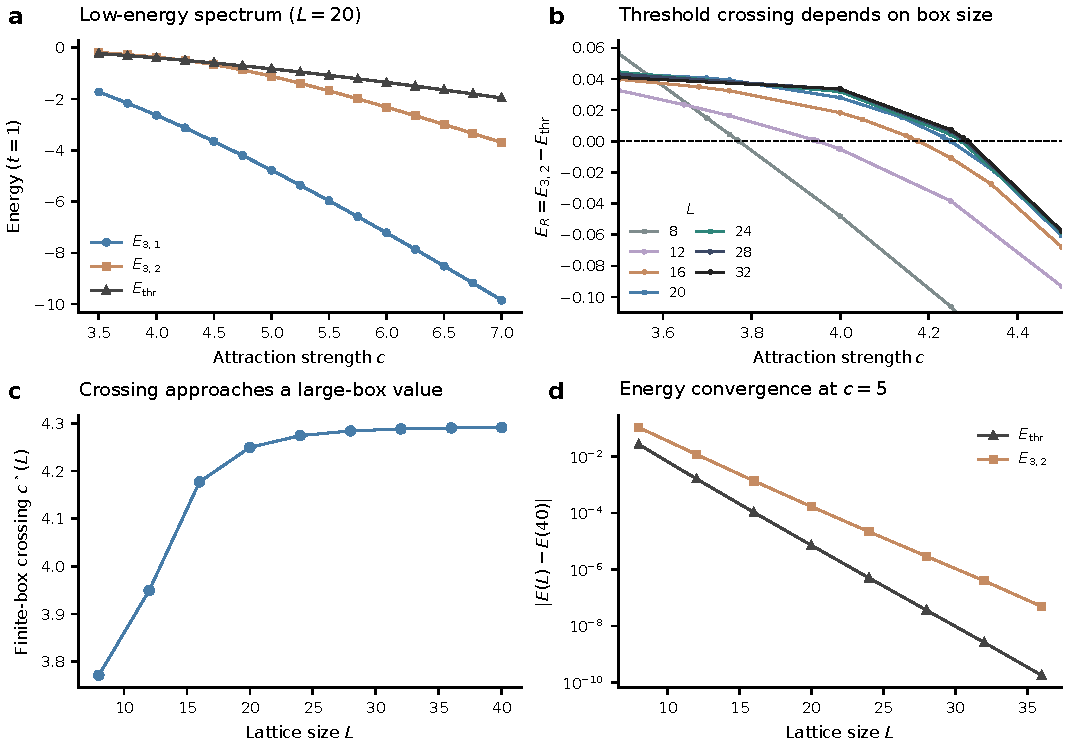
\includegraphics[width=\textwidth]{../figures/spectrum_convergence.pdf}
\caption{\textbf{a} Levels at $L=20$ decrease monotonically with $c$. \textbf{b} $E_R(c)$ crosses zero from above; the crossing shifts right with $L$.
\textbf{c} $c^\star(L)$ approaches a plateau. \textbf{d} Difference from $L=40$ at $c=5$, decaying exponentially.}
\label{fig:spectrum}
\end{figure}

\subsection{Finite volume and the crossing}\label{sec:fv}
\begin{table}[H]
\centering\small
\begin{tabular}{rrrrr}\toprule $L$ & $E_2$ ($c=5$) & $E_{3,1}$ ($c=5$) & $E_{3,2}$ ($c=5$) & $c^\star(L)$ \\ \midrule
8 & -0.847376048 & -4.771681772 & -1.214088937 & 3.7717075 \\
12 & -0.822388617 & -4.771434751 & -1.120646222 & 3.9493804 \\
16 & -0.820874284 & -4.771434367 & -1.110186317 & 4.1770508 \\
20 & -0.820776322 & -4.771434366 & -1.108993749 & 4.2494228 \\
24 & -0.820769644 & -4.771434366 & -1.108848047 & 4.2741346 \\
28 & -0.820769174 & -4.771434366 & -1.108829219 & 4.2838791 \\
32 & -0.820769140 & -4.771434366 & -1.108826687 & 4.2881251 \\
36 & -0.820769138 & -4.771434366 & -1.108826337 & 4.2901120 \\
40 & -0.820769138 & -4.771434366 & -1.108826287 & 4.2910935 \\
\bottomrule\end{tabular}

\caption{Energies at $c=5$ and the crossing point for each $L$.}
\end{table}
\begin{itemize}
\item The compact ground state is stable to 9 decimals for $L\ge20$; the threshold and Hoyle-like state converge more slowly; $c^\star(L)$ slowest of all.
\item $c^\star$ rises from 3.77 ($L=8$) to \CstarMax\ ($L=\Lmax$); the last step changes it by only \LastRootChange, still far above the root tolerance $2\times10^{-7}$.
      The precision is thus limited by finite volume:
      \[\boxed{c^\star\approx4.29}\]
\item $L=20$ suffices for the benchmark but underestimates the crossing as 4.249.
\end{itemize}

\subsection{Spatial structure: why the Hoyle-like state is more sensitive}
Pair distribution $P(\rr_1)=\sum_{\rr_2}|\psi|^2$ and RMS separation $r_{\rm rms}=[\sum d_L(\rr_1)^2P(\rr_1)]^{1/2}$:
ground state $\RmsGround\,a$, Hoyle-like state $\RmsExcited\,a$, about three times larger, consistent with the finite-volume argument of Sec.~\ref{sec:analytic}.
\begin{figure}[H]
\centering
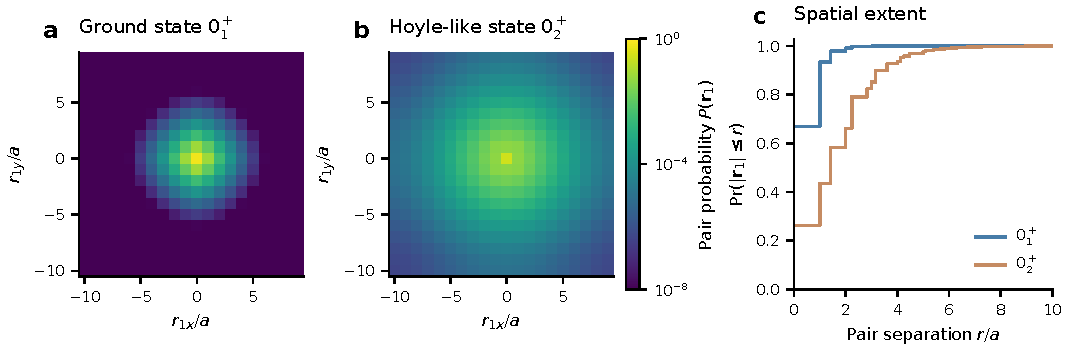
\includegraphics[width=\textwidth]{../figures/state_structure.pdf}
\caption{$c=5,L=20$. \textbf{a,b} Pair distributions of the two states (common log scale). \textbf{c} Cumulative probability of the pair separation.}
\end{figure}

%====================================================================
\section{Conclusions}
\begin{enumerate}
\item Starting from the single-particle hopping rule and translation invariance, we derived the Hamiltonians in relative coordinates for two bodies (amplitude $2t$) and three bodies (including the diagonal hop of particle 3).
\item Lanczos in the full space plus a test against the $S_3\times D_4$ generators yields $0^+_1,0^+_2$ and reproduces the benchmark.
\item All levels fall with $c$; the Hoyle-like state falls faster and crosses the threshold at $c^\star\approx4.29$, which needs $L\gtrsim28$ to be stable within $10^{-2}$.
\item The analytic free spectrum, symmetry commutators, Hellmann--Feynman, the residual bound and $L$ convergence test the derivation, the implementation and the box size respectively.
\end{enumerate}
\textbf{Scope:} a lattice model at fixed spacing $a=1$, with no continuum limit; discrete finite-box levels are not the same as infinite-volume resonances.

\end{document}
